\chapter {Automação Residencial}
\label{cap:1}

\section {Considerações Iniciais}
De acordo com \citeonline{groover1987}, automação é a tecnologia pela qual um processo é realizado
sem assistência humana através de um sistema de controle, instruções de programa e alguma forma de energia,
sendo a elétrica a mais comum.

Seguindo esta mesma definição, uma automação residencial é um produto ou serviço que proporciona algum nível de
ação ou mensagem para o ambiente domiciliar, um evento que foi gerado sem a intervenção direta do morador. Um
despertador ou um alarme de incêndio são exemplos disso, porém, esses dispositivos autônomos não
necessariamente possuem um mecanismo de comunicação entre eles, limitando o nível da automação e inteligência
da solução. \cite{riley2012}

A automação residencial é um componente fundamental para que se possa construir casas inteligentes, ou seja,
ambientes inteligentes que interagem dinamicamente e respondem prontamente às necessidade dos ocupantes a às
mudanças condicionais de uma maneira adaptativa. \cite{al-qutayri2010}

A variedade de aplicações suportadas por uma casa inteligente é bastante abrangente. Algumas das mais comuns incluem
monitoramento e controle do ambiente, segurança, entretenimento, serviços baseados em localização, cuidados
de crianças e idodos, entre outros. \cite{al-qutayri2010}

É desejável que essa automação seja pervasiva, ou seja, que a interação entre o usuário e o ambiente ocorra
naturalmente. Os dispositivos de uma solução pervasiva, ou ubíqua, possuem três características fundamentais:
miniaturalização, comunicação e autonomia. \cite{lalanda2010}

O atendimento desses critérios está ocorrendo de uma forma crescente nos últimos anos através da evolução dos
equipamentos computacionais, tornando ainda mais acessível o desenvolvimento de uma automação residencial,
seja por empresas ou entusiastas na área.

\section{Conceitos Chaves}
Para \citeonline{kyas2013}, uma automação residencial consiste em cinco blocos de construção:

\begin{itemize}
	\item Dispositivos sob controle;
	\item Dispositivos de controle remoto;
	\item Rede de controle;
	\item Controlador;
	\item Sensores e atuadores.
\end{itemize}

\subsection{Dispositivos Sob Controle}
Trata-se dos eletrodomésticos pertencentes à uma residência, como geladeira, televisão, etc. Atualmente,
esses dispositivos já possuem diversas funcionalidades embutidas, podendo ser chamados de inteligentes por si
só.

Um grande exemplo são as \textit{smart TVs}, que possibilitam com que a televisão deixe de ser apenas um
aparelho de reprodução de conteúdo para ser um centro de entretenimento interativo.

Ainda há muito a se explorar nessa área de aparelhos de consumo inteligentes. Teoriza-se possível, por
exemplo, oferecer ao consumidor um mecanismo para comprar objetos e roupas que estão sendo exibidos em
determinado filme, ou então controlar o estoque e validade dos alimentos mantidos na geladeira, entre muitas
outras utilidades.

O principal desafio está em integrar todos esses eletrodomésticos ao sistema de automação residencial, sendo
necessário definir um mecanismo de comunicação e adaptar os aparelhos que não o possuam.

\subsection{Dispositivos de Controle Remoto}
São responsáveis por oferecer uma interface remota ao usuário para gerenciar o sistema de automação. Para
isso, eles se conectam ao controlador, seja através da própria rede de controle ou outro meio fornecido, como
a \textit{Internet}. Atualmente esses dispositivos são representados principalmente por \textit{smartphones} e
\textit{tablets}, cuja existência é um dos principais motivos pelo aumento da aceitação de sistemas de
automação em ambientes residenciais. \cite{kyas2013}

\subsection{Rede de Controle}
É quem possibilita a conexão entre os dispositivos sob controle, sensores e atuadores com o controlador e, às
vezes, com os dispositivos de controle remoto. \cite{kyas2013}

Embora existam várias implementações que utilizam fios (sejam eles de energia ou apenas de dados) para
transportar as mensagens, a comunicação sem fio é a melhor alternativa para obter uma solução ubíqua, além de
normalmente ter um custo de desenvolvimento e implantação muito menor.

\subsection{Controlador}
É um sistema computacional onde se localiza a aplicação de controle da automação. É responsável por receber comandos do
usuário e interagir com os dispositivos e transdutores.

Qualquer computador pessoal pode assumir esta função, mas normalmente se utiliza microcomputadores de pequeno porte com sistema
operacional embarcado devido ao baixo preço e baixo consumo elétrico que eles proporcionam.

Um dos principais exemplos de microcomputadores dessa categoria é o \textt{Raspberry Pi}, ilustrado na figura
\ref{figura:pi}. Foi desenvolvido inicialmente com o propósito de ensinar crianças a programar, porém ganhou uma
imensa aceitação e passou a ser utilizado para diversos propósitos, como centro multimídia, servidor
\textit{web}, e, principalmente, para experimentação com eletrônicos. \cite{schmidt2014}

\begin{figure}[h]
	\centering
	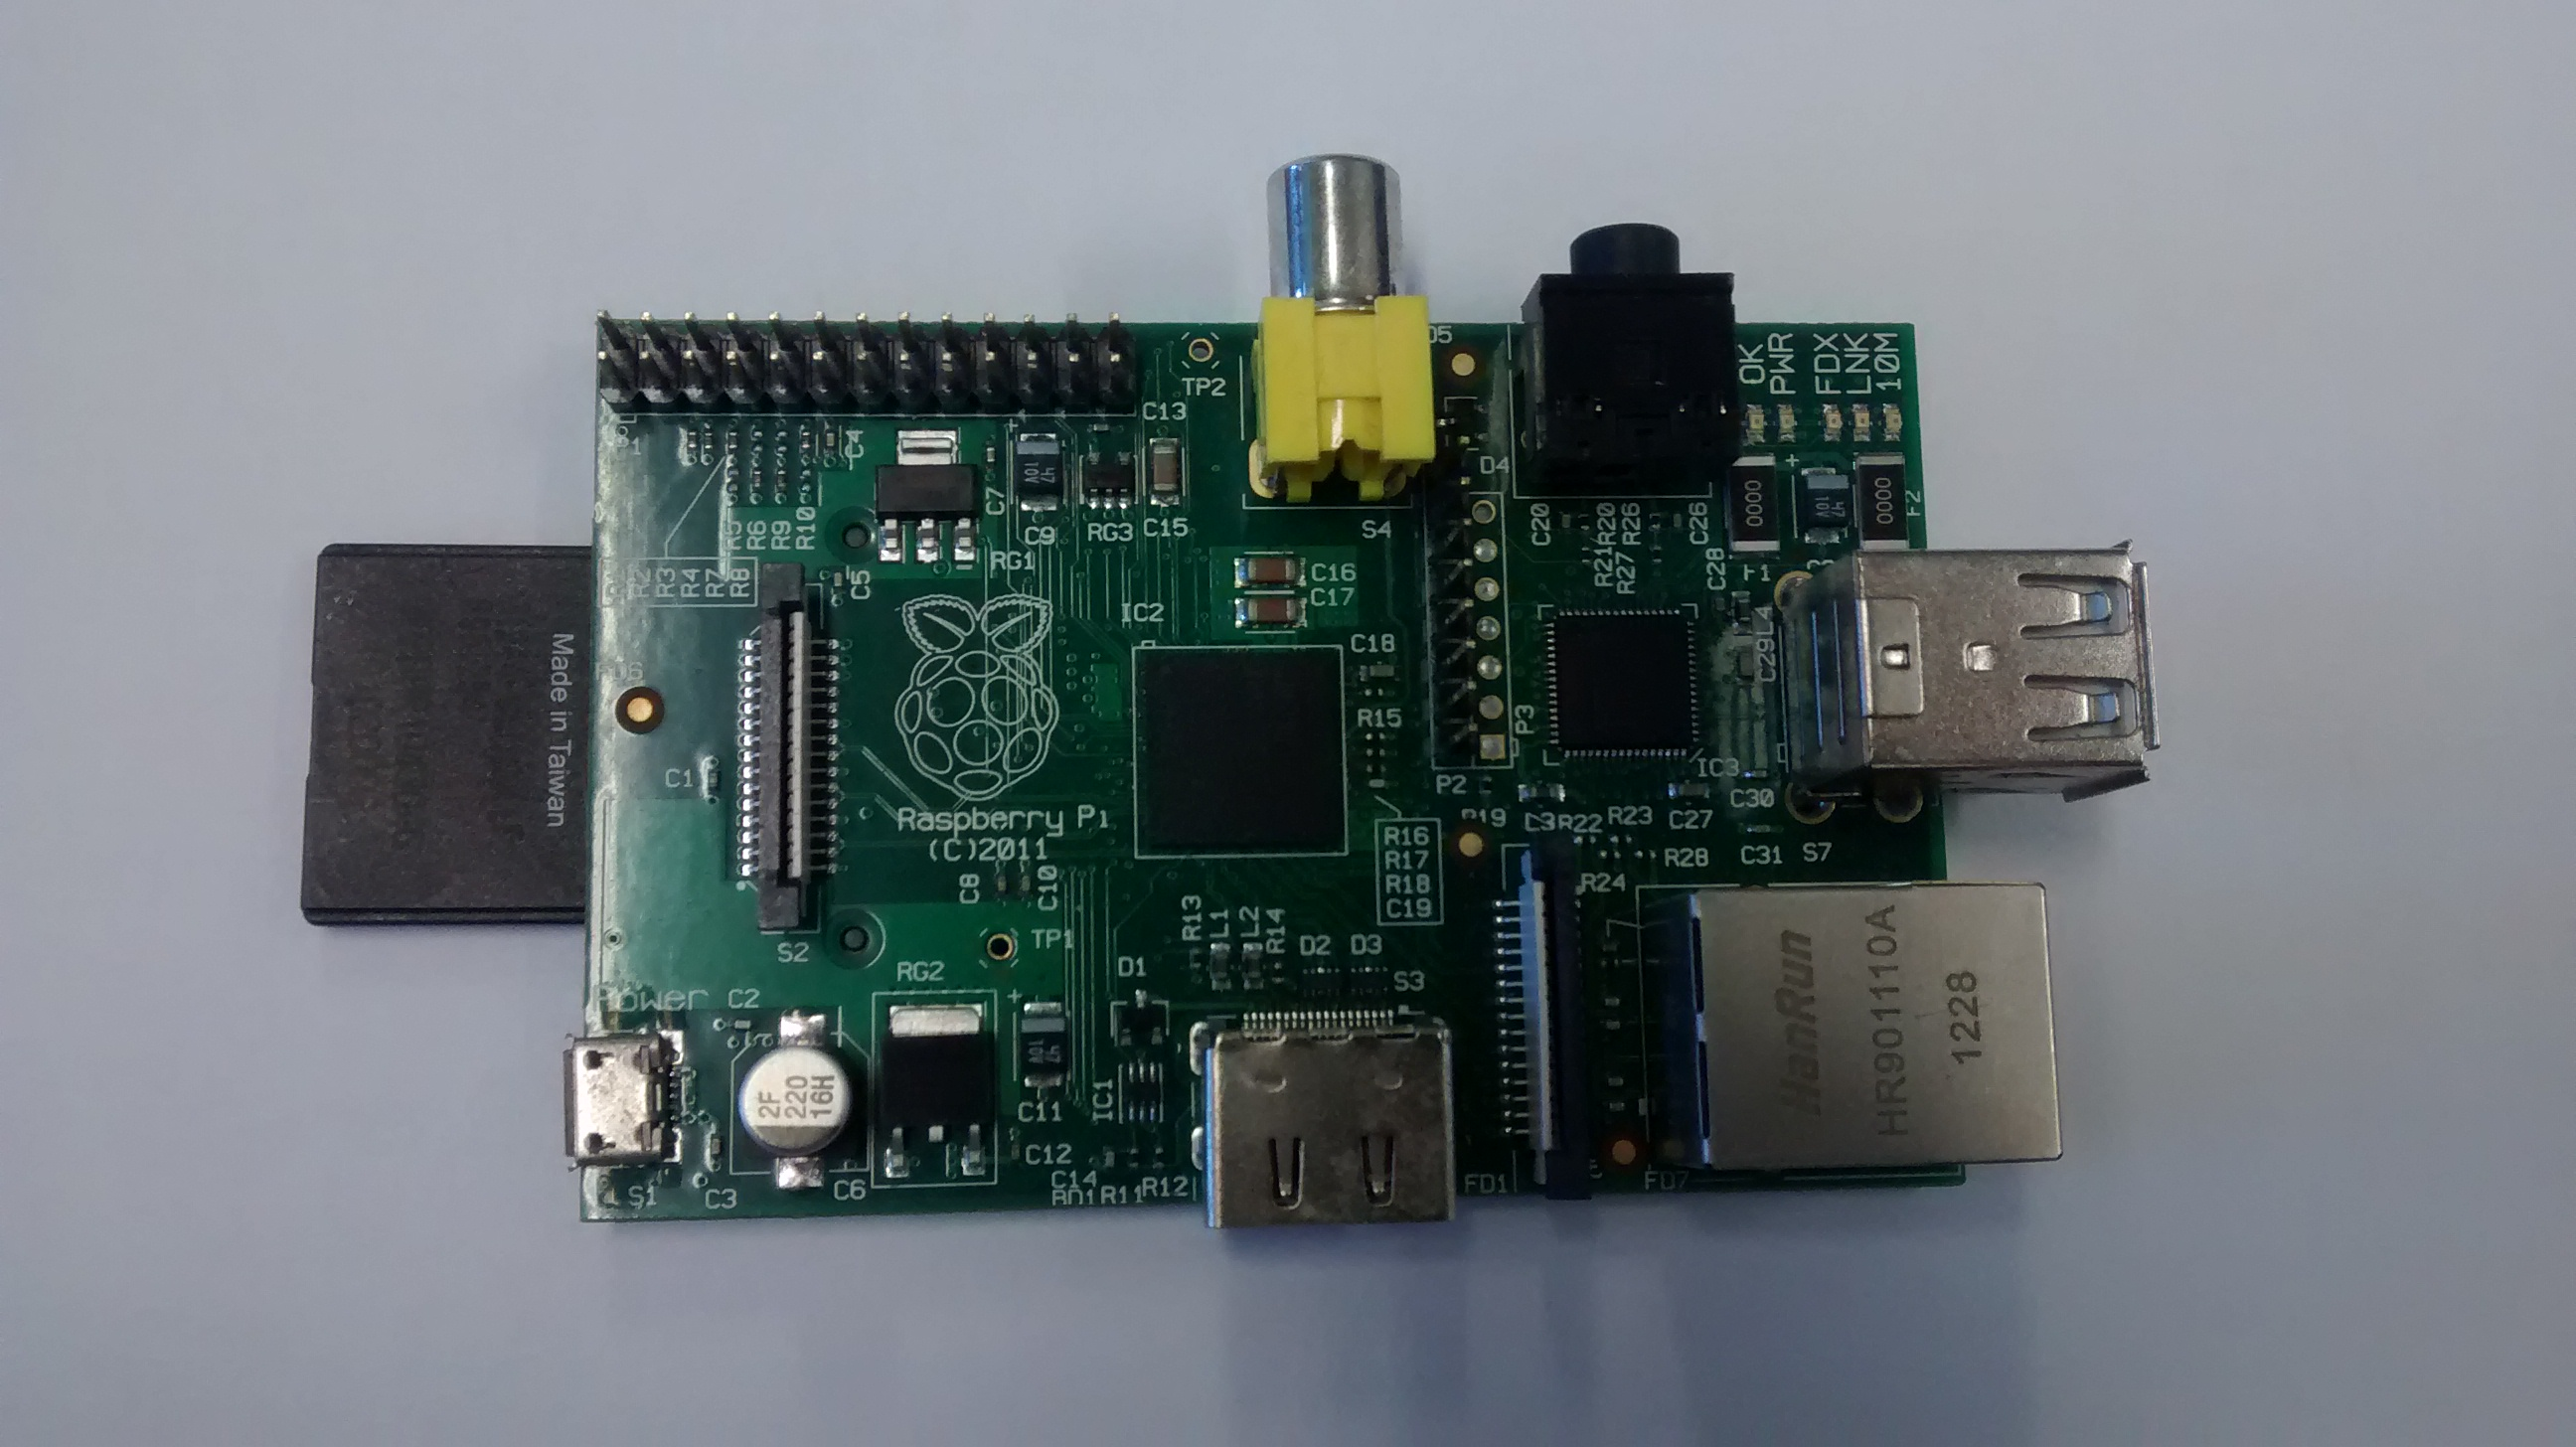
\includegraphics[width=300]{../images/raspeberry.jpg}
	\caption{Raspberry Pi}
	\label{figura:pi}
\end{figure}

\subsection{Sensores e Atuadores}


\section{Desafios}

\section {Considerações Finais}
